\documentclass{article}\usepackage[]{graphicx}\usepackage[]{color}
%% maxwidth is the original width if it is less than linewidth
%% otherwise use linewidth (to make sure the graphics do not exceed the margin)
\makeatletter
\def\maxwidth{ %
  \ifdim\Gin@nat@width>\linewidth
    \linewidth
  \else
    \Gin@nat@width
  \fi
}
\makeatother

\definecolor{fgcolor}{rgb}{0.345, 0.345, 0.345}
\newcommand{\hlnum}[1]{\textcolor[rgb]{0.686,0.059,0.569}{#1}}%
\newcommand{\hlstr}[1]{\textcolor[rgb]{0.192,0.494,0.8}{#1}}%
\newcommand{\hlcom}[1]{\textcolor[rgb]{0.678,0.584,0.686}{\textit{#1}}}%
\newcommand{\hlopt}[1]{\textcolor[rgb]{0,0,0}{#1}}%
\newcommand{\hlstd}[1]{\textcolor[rgb]{0.345,0.345,0.345}{#1}}%
\newcommand{\hlkwa}[1]{\textcolor[rgb]{0.161,0.373,0.58}{\textbf{#1}}}%
\newcommand{\hlkwb}[1]{\textcolor[rgb]{0.69,0.353,0.396}{#1}}%
\newcommand{\hlkwc}[1]{\textcolor[rgb]{0.333,0.667,0.333}{#1}}%
\newcommand{\hlkwd}[1]{\textcolor[rgb]{0.737,0.353,0.396}{\textbf{#1}}}%
\let\hlipl\hlkwb

\usepackage{framed}
\makeatletter
\newenvironment{kframe}{%
 \def\at@end@of@kframe{}%
 \ifinner\ifhmode%
  \def\at@end@of@kframe{\end{minipage}}%
  \begin{minipage}{\columnwidth}%
 \fi\fi%
 \def\FrameCommand##1{\hskip\@totalleftmargin \hskip-\fboxsep
 \colorbox{shadecolor}{##1}\hskip-\fboxsep
     % There is no \\@totalrightmargin, so:
     \hskip-\linewidth \hskip-\@totalleftmargin \hskip\columnwidth}%
 \MakeFramed {\advance\hsize-\width
   \@totalleftmargin\z@ \linewidth\hsize
   \@setminipage}}%
 {\par\unskip\endMakeFramed%
 \at@end@of@kframe}
\makeatother

\definecolor{shadecolor}{rgb}{.97, .97, .97}
\definecolor{messagecolor}{rgb}{0, 0, 0}
\definecolor{warningcolor}{rgb}{1, 0, 1}
\definecolor{errorcolor}{rgb}{1, 0, 0}
\newenvironment{knitrout}{}{} % an empty environment to be redefined in TeX

\usepackage{alltt}
\usepackage{Sweave}
\usepackage{float}
\usepackage{graphicx}
\usepackage{tabularx}
\usepackage{siunitx}
\usepackage{geometry}
\usepackage{pdflscape}
\usepackage{mdframed}
\usepackage{natbib}
\bibliographystyle{..//refs/styles/besjournals.bst}
\usepackage[small]{caption}
\setlength{\captionmargin}{30pt}
\setlength{\abovecaptionskip}{0pt}
\setlength{\belowcaptionskip}{10pt}
\topmargin -1.5cm        
\oddsidemargin -0.04cm   
\evensidemargin -0.04cm
\textwidth 16.59cm
\textheight 21.94cm 
%\pagestyle{empty} %comment if want page numbers
\parskip 7.2pt
\renewcommand{\baselinestretch}{1.5}
\parindent 0pt
\usepackage{lineno}
\linenumbers

\newmdenv[
  topline=true,
  bottomline=true,
  skipabove=\topsep,
  skipbelow=\topsep
]{siderules}

%% R Script


\IfFileExists{upquote.sty}{\usepackage{upquote}}{}
\begin{document}
\title{Rethinking False Spring Risk}
\author{C. J. Chamberlain $^{1,2}$, B. I. Cook $^{3}$, I. Garcia de Cortazar Atauri $^{4}$ \& E. M. Wolkovich $^{1,2}$}
\date{\today}
\maketitle 
%\tableofcontents
 

\renewcommand{\thetable}{\arabic{table}}
\renewcommand{\thefigure}{\arabic{figure}}
\renewcommand{\labelitemi}{$-$}
\setkeys{Gin}{width=0.8\textwidth}

%%%%%%%%%%%%%%%%%%%%%%%%%%%%%%%%%%%%%%%%%%%%%%%
% General to do
% Move all figures and their captions to end of manuscript
% Work on transitions throughout. I made note of it many places.
% My comments are usually in [] and I made some edits throughout. You can use the app FileMerge (spotlight search for it) on most Macs to see the changes quickly. 
%%%%%%%%%%%%%%%%%%%%%%%%%%%%%%%%%%%%%%%%%%%%%%%


\section{Abstract}
Temperate trees and shrubs are at risk of being exposed to late spring freezes --- often called false spring events --- which can be damaging ecologically and economically. As climate change may alter the potential prevalence and severity of false spring events, our ability to accurately forecast such events has become more critical. Yet currently, many false spring studies simplify the various ecological elements needed for accurate predictions of the level of plant damage from late spring freezing events. Here we review the complexity of factors driving a plant's false spring risk. We highlight how species, life stage, and habitat differences contribute to the likelihood of occurrence and damage potential of false spring events. %(The ultimate intent is to demonstrate how an integrated view of false spring that incorporates these factors would rapidly advance progress in this field.)
%EMW: You mention equation above, but have not told the audience about any equations, re-work the sentence/paragraph (probably best to remove 'equation').
Integrating some of these complexities could help rapidly advance understanding and forecasting of false spring events in climate change and ecological studies.
% In this paper we aim to highlight the complexity of factors driving a plant's false spring risk and provide a road map for improved metrics. First, we review the currently used definitions of false spring. Then, combining research from plant physiology, climatology and community ecology, we outline major gaps in current definitions.

\section{Introduction}

Plants growing in temperate environments time their growth each spring to follow rising temperatures alongside increasing light and soil resource availability. While tracking spring resource availability, temperate plants are at risk of late spring freezes, which can be detrimental to growth. Individuals that leaf out before the last freeze date are at risk of leaf loss, damaged wood tissue, and slowed or stalled canopy development \citep{Gu2008, Hufkens2012}. These damaging late spring freezing events are also known as false springs, and are widely documented to result in highly adverse ecological and economic consequences \citep{Knudson2012, Ault2013}.

% EMW: Thanks for adding references to the temperature variation. Unfortunately I am not comfortable with these references, especially the Vasseur one (remind me and we can discuss briefly). I suggest you remove this one and add 1-2 from the climate literature. My understanding is temperature variation is not going to change that much in most regions, and I don't want to support a narrative that it will when it won't. An easy fix for now is deleting a couple sentences I am not sure we need (deleted below, see what you think). But in the longer run I suggest you Skype with Ben to discuss more and track down some balanced citations from the physical science literature.
Climate change is expected to cause an increase in damage from false spring events due to earlier spring onset and potentially greater fluctuations in temperature in some regions \citep{Cannell1986, Inouye2008, Martin2010}. Already, multiple studies have documented false spring events in recent years \citep{Gu2008, Augspurger2009, Knudson2012, Augspurger2013} and some have linked these events to climate change \citep{Ault2013, Allstadt2015, Muffler2016, Xin2016}. This increasing interest in false spring events has led to a growing body of research investigating the effects on temperate forests and agricultural crops. But for this research to produce accurate predictions of future trends, researchers need methods that properly evaluate the effects of false spring events across the diverse species, habitats and climate regimes they are studying. 

Current metrics for estimating false springs events are generally simple, often requiring an estimate for the start of biological `spring' (i.e. budburst) and whether temperatures occurred below a particular temperature threshold in the following week. Such estimates inherently assume consistency of damage across species, functional group, life stages, habitat type, and other climatic regimes, ignoring that such factors can greatly impact plants' false spring risk. As a result, such indices may lead to inaccurate current estimates as well as poor future predictions, slowing our progress in understanding false spring events and how they may shift with climate change. 

In this paper we highlight the complexity of factors driving a plant's false spring risk and provide a road map for improved metrics. We show how life stage, location within a forest or canopy, interspecific variation in avoidance and tolerance strategies, freeze temperature thresholds, and regional effects unhinge simple metrics of false spring. We argue that a new approach that integrates these and other crucial factors would help accurately determine current false spring damage and improve predictions of spring freeze risk under a changing climate --- while potentially providing novel insights to how plants respond to and are shaped by spring frost. % The ultimate intent is to demonstrate how an integrated view of false spring that incorporates these factors would rapidly advance progress in this field.  

\section{Defining False Spring: An example in one temperate plant community}
Temperate forest plants experience elevated risk of frost damage during the spring due to the stochastic timing of spring frosts. 
% Temperate forest plants are most at risk to frost damage from episodic spring frosts \citep{Sakai1987}. 
Plants must therefore exhibit flexible spring phenologies to minimize freezing risk. Freezing temperatures following a warm spell could result in plant damage or even death \citep{Ludlum1968, Mock2007}. Intracellular ice formation from false spring events, for example, often results in severe leaf and stem damage \citep{Burke1976, Sakai1987}. Ice formation can also occur indirectly (i.e. extracellularly), which results in freezing dehydration and mimics extreme drought conditions \citep{Pearce2001, Beck2004, Hofmann2015}. Both forms of ice formation can cause defoliation and, ultimately, crown dieback \citep{Gu2008}. Once buds exit the dormancy phase, they are less freeze tolerant and resistance to bud ice formation is greatly reduced \citep{Taschler2004, Lenz2013, Vitasse2014a}. An effective and consistent definition of false spring would accurately determine the amount and type of ice formation to properly evaluate the level of damage that could occur.

% EMW: Tiny edits below...
There are several definitions currently used to define a false spring. A common definition describes a false spring as having two phases: rapid vegetative growth prior to a freeze and a post freeze setback \citep{Gu2008}. Other definitions instill more precise temporal parameters, specific to certain regions \citep[e.g., in][false spring for the Midwestern United States is defined as a warmer than average March, a freezing April, and enough growing degree days between budburst and the last freeze date]{Augspurger2013}. A widely used definition integrates a mathematical equation to quantify a false spring event. This equation, known as a False Spring Index (FSI), signifies the likelihood of damage to occur from a late spring freeze. Currently, FSI is evaluated annually by the day of budburst and the day of last spring freeze (often calculated at -2.2$^{\circ}$C \citep{Schwartz1993}) through the simple equation \citep{Marino2011}:
\begin{equation} \label{eq:1}
FSI = \text{Day of Year} (Last Spring Freeze) - \text{Day of Year} (Budburst)
\end{equation}
Negative values indicate no risk situations, whereas a damaging FSI is currently defined to be 7 or more days between budburst and the last freeze date (Equation \ref{eq:1}) \citep{Peterson2014}. This 7 day threshold captures the reality that leaf tissue is at high risk of damage from frost in the period after budburst, with later vegetative phases (e.g., full leafout) being more resistant to such damage.% OLD: By using the 7 day threshold, it is likely less resistant vegetative phenophases will be exposed to a false spring, thus putting the plant at a higher risk of damage. 

To demonstrate how the FSI definition works, we applied it to data from the Harvard Forest Long-term Ecological Research program in Massachusetts. We used three separate methodologies to calculate spring onset: long-term ground observational data \citep{Okeefe2014}, PhenoCam data from Harvard Forest \citep{Richardson2015}, and USA National Phenology Network (USA-NPN) Extended Spring Index (SI-x) data \citep{USA-NPN2016}. These spring onset values were then inputted into the FSI equation (Equation \ref{eq:1}) to calculate FSI from 2008 to 2014 (Figure \ref{fig:fsifig}). 

% EMW: Tiny edits below...
Each methodology renders different FSI values, suggesting different false spring damage for the same site and same year. For most years, the observational FSI and PhenoCam FSI are about 10-15 days lower than the SI-x data. This is especially important for 2008, when the SI-x data indicates a false spring year, whereas the other two datasets do not. In 2012, the observational data and PhenoCam data diverge and the PhenoCam FSI is over 30 days less than the SI-x value.

The reason for these discrepancies is that each method evaluates spring onset by integrating different attributes (e.g. age, species or functional group). Common functional groups are C3 grasses or early successional broadleaf deciduous trees. Spring phenology in temperate forests typically progresses by functional group: understory species and young trees tend to initiate budburst first, whereas larger canopy species may start later in the season \citep{Richardson2009, Xin2016}. The different FSI values determined in Figure \ref{fig:fsifig} exemplify the differences in functional group spring onset dates and illustrate variations in forest demography and phenology, which is most apparent in 2012. In 2012, a false spring event was reported through many regions of the US due to warm temperatures occurring in March \citep{Ault2015}. These high temperatures would most likely be too early for larger canopy species to initiate budburst but they would affect smaller understory species as is seen in Figure 1. 

% EMW: Tiny edits below...
Yet, in contrast to our three metrics of spring onset for one site, most FSI work currently ignores variation across functional groups --- instead using one metric of spring onset and assuming it applies to the whole community of plants \citep{Marino2011, Peterson2014, Allstadt2015, Mehdipoor2017}. The risk of a false spring varies across habitats and with species composition since spring onset is not consistent across functional groups. Therefore, one spring onset date cannot be used as an effective proxy for all species. False spring studies should first assess the forest demographics and functional groups relevant to the study question in order to effectively estimate the date of spring onset. However, as we outline below, considering different functional groups is unlikely to be enough for robust predictions. It is also crucial to integrate species differences within functional groups and consider the various interspecific avoidance and tolerance strategies that species have against false springs. %EMW cut after re-order: ... equation is built half on spring onset date, it is critical to choose the most appropriate methodology that targets the species of interest within the study. 

\section {Plant Physiology and Diversity versus the Current False Spring Definition}
% EMW: I am not sure the below change I made is needed, but it does keep the cue text a bit closer together.
Plants have evolved to minimize false spring damage through two strategies: avoidance and tolerance. Many temperate forest plants utilize various morphological strategies to be more frost tolerant: some have toothed or lobed leaves to increase `packability' in winter buds, which permits more rapid leafout and minimizes exposure time of less resistant tissues \citep{Edwards2017}. Other species have young leaves with more trichomes to act as a buffer against spring frosts \citep{Agrawal2004, Prozherina2003}, and many are able to respond to abiotic cues such as consistently dry winters. Species living in habitats with drier winters develop shoots and buds with decreased water content, which makes the buds more tolerant to drought and also to false spring events \citep{Beck2007, Morin2007, Nielsen2009, Poirier2010, Kathke2011, Hofmann2015}. More studies are needed to investigate the interplay between false spring events, leaf morphology, and drought tolerance and how these relationships affect false spring tolerance. 

Rather than being more tolerant of spring freezing temperatures, some temperate forest species have evolved to avoid frosts via more flexible phenologies. Effective avoidance strategies require well-timed spring phenologies. Temperate deciduous tree species optimize growth and minimize spring freeze damage by using three cues to initiate budburst: low winter temperatures, warm spring temperatures, and increasing photoperiods \citep{Chuine2010}. The evolution of these three cues and their interactions has permitted temperate plant species to occupy more northern ecological niches and decrease the risk of false spring damage, which is crucial for avoidance strategies \citep{Samish1954}. One avoidance strategy, for example, is the interaction between over-winter chilling and spring forcing temperatures. Warm temperatures earlier in the year (i.e. in February, or even January in the Mediterranean) will not result in early budburst due to insufficient chilling \citep{Basler2012}. Likewise, photoperiod sensitivity is a common false spring avoidance strategy: species that respond strongly to photoperiod cues in addition to warm spring temperatures will likely delay budburst and evade false spring events as spring continues to advance earlier in the year \citep{Basler2014}. 
% Given the diverse array of spring freezing defense mechanisms, predicting damage by false spring events requires a greater understanding of avoidance and tolerance strategies across species, especially with a changing climate.

\section {Defining Vegetative Risk} % Complexities due to Species' Strategies and Climate
Phenology and frost tolerance are intertwined --- with important variation occurring across different phenological phases. Flowering and fruiting are generally more sensitive to false spring events than vegetative phases \citep{Augspurger2009, Lenz2013}.
However, false spring events that occur during the vegetative growth phenophases may impose the greatest freezing threat to deciduous tree and shrub species. Plants will suffer greater long-term effects from the loss of photosynthetic tissue compared to floral and fruit tissue, which could impact multiple years of growth, reproduction, and canopy development \citep{Sakai1987, Vitasse2014}. 

There is also important variation within certain phenological phases. Most notably, within the vegetative phases of spring leafout, plants that have initiated budburst but have not fully leafed out are more likely to sustain damage from a false spring than individuals past the leafout phase. This is because freezing tolerance steadily decreases after budburst begins until the leaf is fully unfolded \citep{Lenz2016} (Figure \ref{fig:risk}). Therefore, the rate of budburst and the length of time between budburst and leafout is essential for predicting level of damage from a false spring event. We will refer to the timing of these phenophases --- budburst (i.e. BBCH 7) to leafout (i.e. BBCH 11 \citep{Meier2001}) --- as the duration of vegetative risk. The duration of vegetative risk is usually extended if a freezing event occurs during the phenophases between budburst and full leafout \citep{Augspurger2009}, which could result in exposure to multiple frost events in one season.

\section {How Species' Phenological Cues Shape Vegetative Risk}
% I suggest several big changes to Fig 6:
% (1) Consider moving it and the text up (as shown here) as in line with I?aki's comment.
% (2) Make panel b the first panel and adjust the current-panel-a to show an easier to explain and defend climate change scenario: high force/low chill (no additional) versus low force/high chill (30 d at 1.5) -- use the 12 hour photoperiod in both examples. Make the current-panel-a become panel-b. See text below for how this would work and let me know what you think
Predictions of false spring critically depend on understanding what controls the duration of vegetative risk across species. For temperate species, the three major cues that control budburst \citep[e.g., low winter temperatures, warm spring temperatures, and increasing photoperiods]{Chuine2010} probably play a dominant role. One study, which examined how these cues impact budburst and leafout, shows that the duration of vegetative risk can vary by 21 days or more depending on the suite of cues a plant experiences (Figure \ref{fig:dan}). The experiment examined 9 temperate trees and shrubs using a fully crossed design of three levels of chilling (field chilling, field chilling plus 30 days at either 1 or 4 $^{\circ}$C), two levels of forcing (20$^{\circ}$C/10$^{\circ}$C or 15$^{\circ}$C/5$^{\circ}$C day/night temperatures) and two levels of photoperiod (8 versus 12 hour days) resulting in 12 treatment combinations. Increased forcing, daylength and chilling all decreased the duration of vegetative risk with forcing causing the greatest decrease (10 days), followed by daylength (9 days), and chilling (2-3 days depending on the temperature), but the full effect of any one cue depended on the other cues due to important interactions---for example, the combined effect of warmer temperatures and longer days would be 14 days, because of -5 days interaction between the forcing and photoperiod cues. 

Such cues may provide a starting point for predicting how climate change will alter the duration of vegetative risk. Robust predictions will require much more information, especially the emissions scenario realized over coming decades \citep{IPCC2014}, but one potential outcome is that higher temperatures will increase forcing and decrease chilling in many locations. Under this scenario experimental results suggest a 11 day decrease in duration of vegetative risk (Figure \ref{fig:dan}A). 
% May need to change next sentence depending on what we say just above... 
This cue interaction could potentially lead to longer durations of vegetative risk than if chilling conditions were not expected to decrease and, thus, expose at risk plants to more intense false spring events or even multiple events in one year. 

Considering the interaction of cues and climate change further complicates understanding species future vulnerabilities to false spring events. Most species are expected to begin leafout earlier in the season with earlier warming spring temperatures but some species may have the opposite response due to less winter chilling or decreased photoperiod cues \citep{Cleland2006, Yu2010, Xin2016}. For example, as climate change progresses, higher spring forcing temperatures may be required for species experiencing insufficient winter chilling (due to warmer winter temperatures), especially at lower latitudes \citep{McCreary1990, Morin2009, Fu2012, Polgar2014, Chuine2010}. Generally, individuals that initiate budburst earlier in the spring may attempt to limit freezing risk by decreasing the duration of vegetative risk in order to minimize the exposure of less frost tolerant phenophases. But with a changing climate and thus shifts in phenological cues (warm temperatures, winter chilling and photoperiod), this relationship may change. Further studies are essential to understand the interplay between chilling, forcing, and photoperiod cues on the duration of vegetative risk, especially for species occupying ecological niches more susceptible to false spring events. 

% This interaction of cues --- and how climate change will affect that interaction --- is crucial for recognizing which species will likely become more at risk of false spring events in the future. 

% Though chilling showed a smaller impact (CITE fig panel a -- effect sizes), it could still have an important impact on shifting the duration of vegetative risk depending on how climate change impacts chilling. In many locations climate change is expected to decrease chilling (cite FU or many others), however, in some locations higher winter temperatures may actually increasing chilling (cite Guy et al. 2014).

% With a changing climate, forcing temperatures may increase and lead to budburst earlier in the season (Figure \ref{fig:dan}B.) while photoperiod at the time of budburst will decrease \citep{Basler2014}. 
% Thus, with greater forcing or longer daylengths, the rate of leafout is expected to accelerate development between budburst and leafout leading to shorter duration of vegetative risk (Figure \ref{fig:dan}B.). 

% OLD: We compared 11 temperate forest species between two treatments: high chilling hours, long photoperiod and high forcing temperatures (strong treatment effects) against no additional chilling, short photoperiod and low forcing temperatures (weak treatment effects) (Flynn and Wolkovich, 2017?). According to the results, all individuals have longer durations of vegetative risk with the weaker treatment effects (Figure \ref{fig:dan}A.) 

% SIDE NOTE: 
% We wrote 'This appears mainly due to forcing temperatures and photoperiod cues, which showed larger effects on the duration of vegetative risk than chilling ... This could suggest that chilling influences budburst and leafout similarly, while photoperiod and forcing temperatures have varying effects on the two phenophases....' but if you look at Dan Flynn's paper and compare Figure 1 leafout and budburst cues you should be able to say EXACTLY why you see the effects do you: you can see that the chilling effects on budburst and leafing are very similar -- this means chilling would not affect DVR too much. Instead you see more forcing and longer photoperiod really speeds up leafout -- more than it speeds up budburst -- so those are the main effects. 

\subsection {Predictable Regional Differences in Climate, Species Responses and False Spring Risk}
Robust predictions must consider the full interplay of species cues and a specific location's climate. A single species may have varying cues across space: various studies that investigate latitudinal effects indicate that species and individuals growing further north respond to a different interaction of cues than those growing further south and, subsequently, species across different regions may have different durations of vegetative risk \citep {Partanen2004, Viheraaarnio2006, Caffarra2011}. Studies also suggest that species within the same system can exhibit different sensitivities to the three cues \citep{Basler2012, Laube2013} thus further amplifying the myriad of climatic and phenological shifts as well as the varying species-level effects.  We assessed climate data across North America and Europe, long-term observational data, and experimental data to gain a better understanding of the the interaction between duration of vegetative risk and false spring events in an attempt to unravel these complexities.

Numerous studies have investigated how the relationship between budburst and major phenological cues varies across space and the genetic variations that occur between populations by using latitudinal gradients \citep{Partanen2004, Viheraaarnio2006, Caffarra2011, Zohner2016, Gauzere2017}. Few, however, have integrated longitudinal variation or regional effects. Yet climate and thus false spring risk and phenological cues vary across regions. For example, consider five different regions within a temperate climate (Figure \ref{fig:regional}). Some regions may experience harsher winters and greater temperature variability throughout the year, and these more variable regions often have a much higher risk of false spring (i.e. Maine) than others (i.e. Lyon) (Figure \ref{fig:regional}). Understanding and integrating such spatiotemporal effects and regional differences when investigating false spring risk and duration of vegetative risk would help improve predictions as climate change progresses.

Accurate predictions need to carefully consider how chilling and forcing cues vary across a longitudinal gradient. Some studies indicate that populations further inland will initiate budburst first, whereas those closer to the coast will initiate budburst later in the season and that the distance from the coast is a stronger indicator of budburst timing than latitude \citep{Myking2007}. Climatic and genetic variation across regions and at different distances from the coast results in varying durations of vegetative risk due to different chilling and forcing temperatures. It is therefore important to recognize climate regime extremes (e.g. seasonal trends, annual minima and annual maxima) across regions in future studies in order to better understand the interplay between duration of vegetative risk and climatic variation. The climatic implications of advancing forcing temperatures could potentially lead to earlier dates of budburst and enhance the risk of frost. These shifts in climatic regimes could vary in intensity across regions (i.e. habitats currently at risk of false spring damage could become low risk regions over time). 

There are also discrepancies in defining a false spring event related to understanding the temperature threshold for damage. Some regions and species may tolerate lower temperature thresholds than others (Figure \ref{fig:temp}). Not only is there debate on what a damaging temperature is, but it is still not well understood how the damage sustained relates to the duration of the frost \citep{Sakai1987, Augspurger2009, Vitasse2014, Vitra2017}. It is crucial to gain an understanding on which climatic parameters result in false spring events and how these parameters may vary across regions. It is anticipated that most regions will have earlier spring onsets, however, last freeze dates will not advance at the same rate \citep{Inouye2008,Martin2010,Labe2016,Sgubin2018}, rendering some regions and species to be more susceptible to false spring events in the future. 

\subsection{Observed Changes in the Duration of Vegetative Risk}
Studies suggest that spring forcing temperatures directly affect the duration of vegetative risk: years with lower forcing temperatures will have longer durations of vegetative risk \citep{Donnelly2017} (Figure \ref{fig:dan}). Therefore, it is hypothesized that the species able to track the shifts in spring advancement due to climate change will be more susceptible to false spring damage \citep{Scheifinger2003}. We investigated this interaction using observational data from Harvard Forest \citep{Okeefe2014} and compared two years of data: one year that was thermally late (1997) and another year that was thermally early (2012).

We found most species in the thermally-early year had longer durations of vegetative risk than those in the thermally-late year. In the thermally-early year, a false spring event was reported across many regions of the US and at Harvard Forest low freezing temperatures were recorded on the 29th of April, after many species had initiated budburst (Figure \ref{fig:hf}). This contrast across years could be due to the less consistent forcing temperatures after budburst in the thermally-early year, the lower photoperiod experienced during the budburst period in the thermally-early year, the false spring event itself (i.e., plants damaged from the false spring may then have taken longer to reach leafout) or it could be a combination of the three depending on the species. Further, the effects of spring forcing temperatures on the duration of vegetative risk varied across species (Figure \ref{fig:hf}), which could indicate variation in physiological cues that drive budburst and influence the duration of vegetative risk.

% Could the below text be moved into a box that discusses dormancy and hardiness?
Temperate trees generally have two phases of dormancy: endodormancy, when trees are inhibited from growing and cold hardiness is greatest, and ecodormancy, when trees can grow if the external environment is conducive \citep{Basler2012}. Chilling cues are considered critical for plants to complete endodormancy and warm temperatures (`forcing') are needed for most plants to exit ecodormancy (Figure \ref{fig:hardiness}). However, it is unclear when precisely plants enter and complete the ecodormancy phase \citep{Chuine2016}, and what temperatures constitute chilling or forcing. With climate change altering temperatures, some research suggests that trees will experience more oscillations between chilling and forcing cues \citep{Martin2010}, and some phenological models suggest that this could extend the number of required growing degree days necessary for budburst to occur \citep{Vitasse2011}.
%

\section{Conclusion}
Temperate forest trees are most at risk to frost damage in the spring due to the stochasticity of spring freezes. With warm temperatures advancing in the spring but last spring freeze dates advancing at a slower rate, there could potentially be more damaging false spring events in the future, especially in high risk regions \citep{Gu2008, Inouye2008}. The current equation for evaluating false spring damage (Equation \ref{eq:1}) largely simplifies the myriad of complexities involved in assessing false spring damage and risks. More studies aimed at understanding relationships between species avoidance and tolerance strategies, climatic regimes, and physiological cue interactions with the duration of vegetative risk would improve predictions. Additionally, research to establish temperature thresholds for damage across functional types and phenophases will help effectively predict false spring risk in the future. An integrated approach to assessing past and future spring freeze damage would offer more robust predictions as climate change progresses, which is essential in order to mitigate the adverse ecological and economic effects of false springs.

\nocite{Soudani2012}
\nocite{White2009}
\nocite{Schaber2005}
\nocite{Schwartz1993}
\nocite{Barker2005}
\nocite{Sanchez2013}
\nocite{Longstroth2012}
\nocite{Barlow2015}
\nocite{Longstroth2013}
\nocite{Charrier2011}
\bibliography{..//refs/SpringFreeze.bib}


\begin{figure}[H]

{\centering 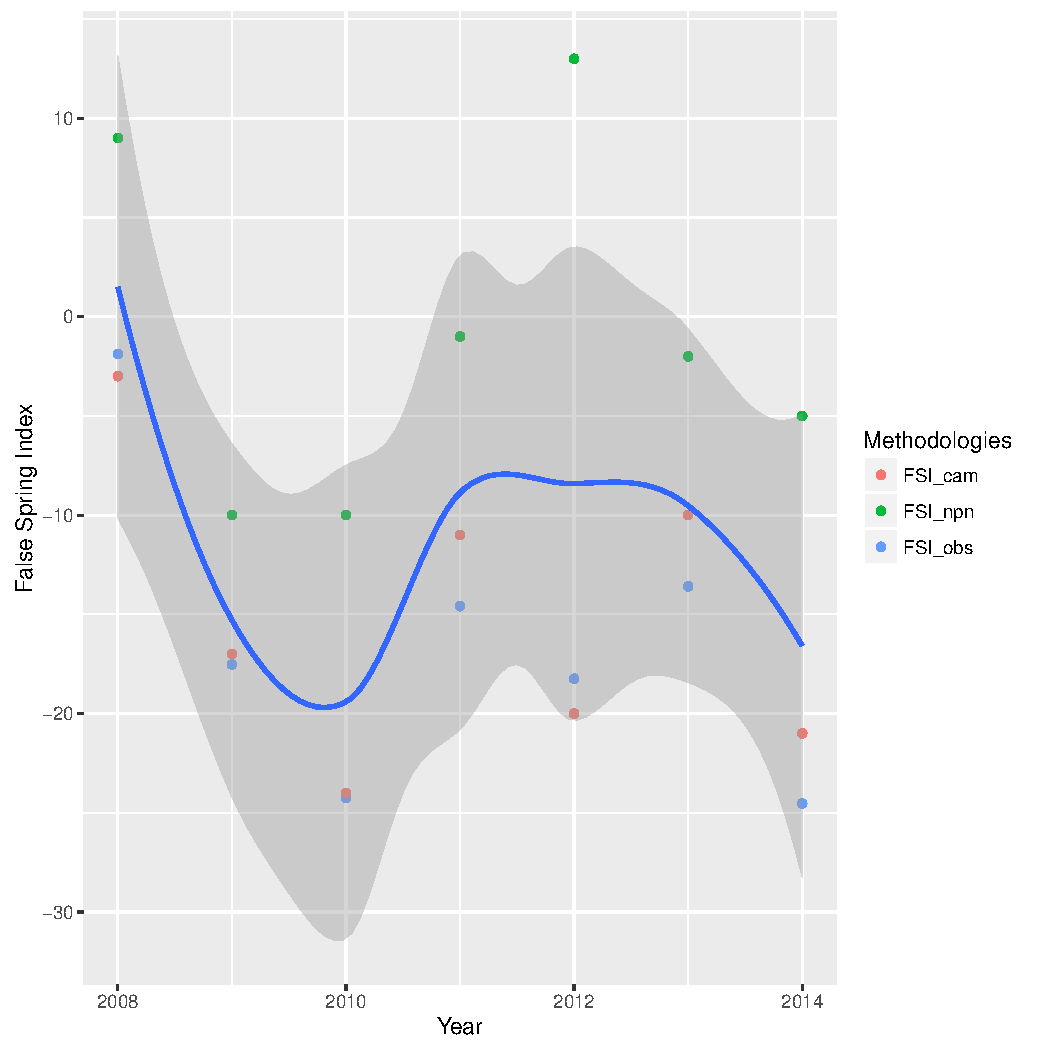
\includegraphics[width=\maxwidth]{figure/fsifig-1} 

}

\caption[A scatterplot indicating FSI values from 2008 to 2014 for each methdology used in this study]{A scatterplot indicating FSI values from 2008 to 2014 for each methdology used in this study. To calculate spring onset, we used the USA-NPN Extended Spring Index tool for the USA-NPN FSI values, which are in red (USA-NPN, 2016), long-term ground observational data for the observed FSI values, which are in green (O'Keefe, 2014), and near-surface remote-sensing canopy data for the PhenoCam FSI values, which are in blue (Richardson, 2015).}\label{fig:fsifig}
\end{figure}



\begin{figure}[H]

{\centering 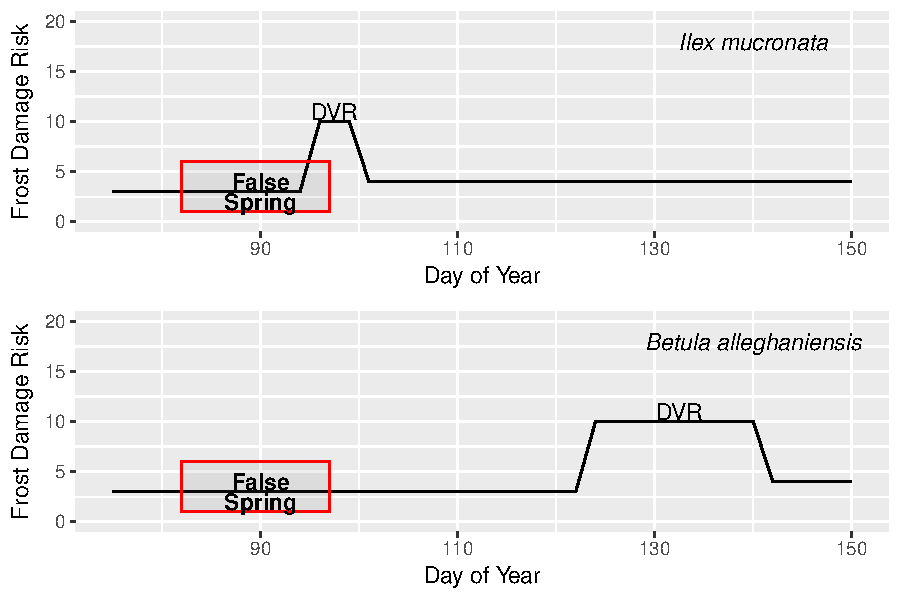
\includegraphics[width=\maxwidth]{figure/risk-1} 

}

\caption{A figure showing the differences in spring phenology and false spring risk across two species: \textit{Ilex mucronata} (L.) and \textit{Betula alleghaniensis} (Marsh.). We mapped a possible false spring event based on historic weather data and compared it to the observational data collected at Harvard Forest (O'Keefe, 2014). In this scenario, the \textit{Ilex mucronata} would be exposed to a false spring event, whereas the \textit{Betula alleghaniensis} would avoid it entirely.}\label{fig:risk}
\end{figure}



\begin{figure} [H] 
 -\begin{center}
 -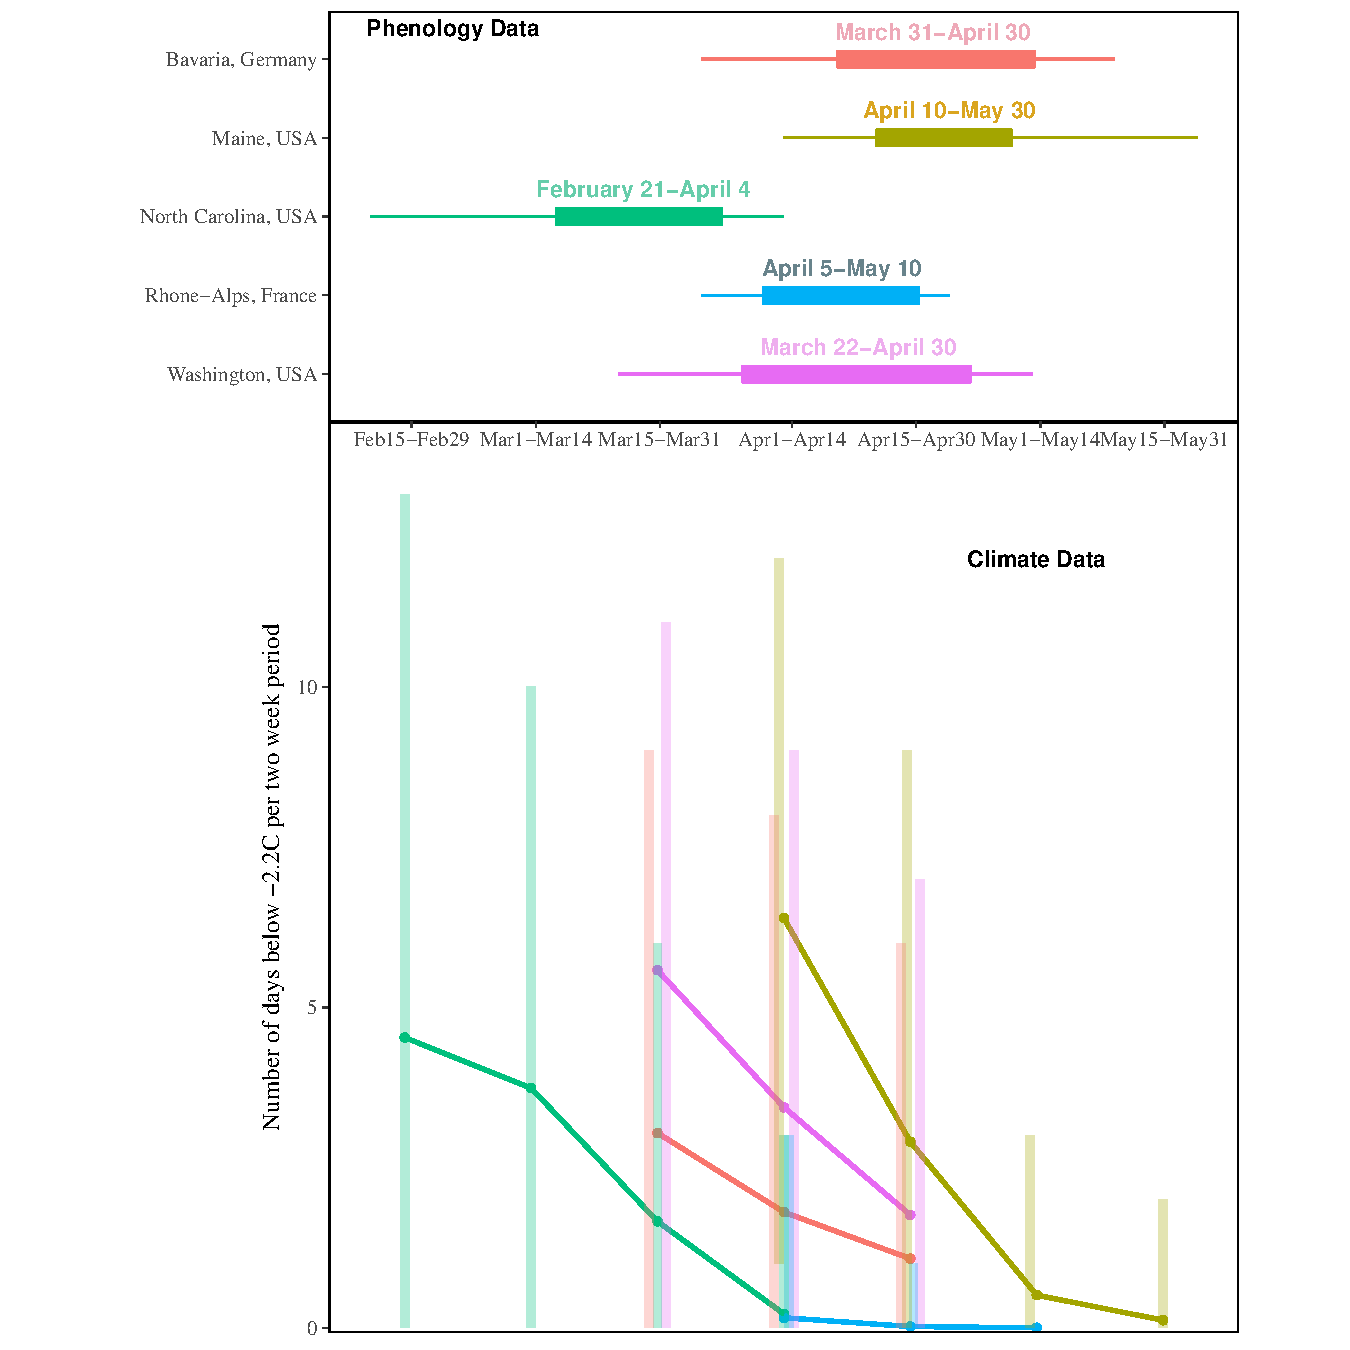
\includegraphics[width=16cm, height=18cm]{..//figure/RegRisk_flipped.pdf} 
 -\caption{False spring risk can vary dramatically across regions. Here we show the period when plants are most at risk to tissue loss -- between budburst and leafout (upper, lines represent the range with the thicker line representing the interquartile range) and the variation in the number of freeze days (-2.2$^{\circ}$C) (Schwartz, 1993) that occurred on average over the past 50 years for five different sites (lower, bars represent the range, points represent the mean). Data come from USA-NPN SI-x tool (1981-2016) and observational studies (1950-2016) for phenology (USA-NPN, 2016; Soudani et al., 2012; White et al., 2009; Schaber \& Badeck, 2005) and NOAA Climate Data Online tool for climate (from 1950-2016). } \label{fig:regional}  
 -\end{center}
 -\end{figure}

\begin{figure}[H]

{\centering 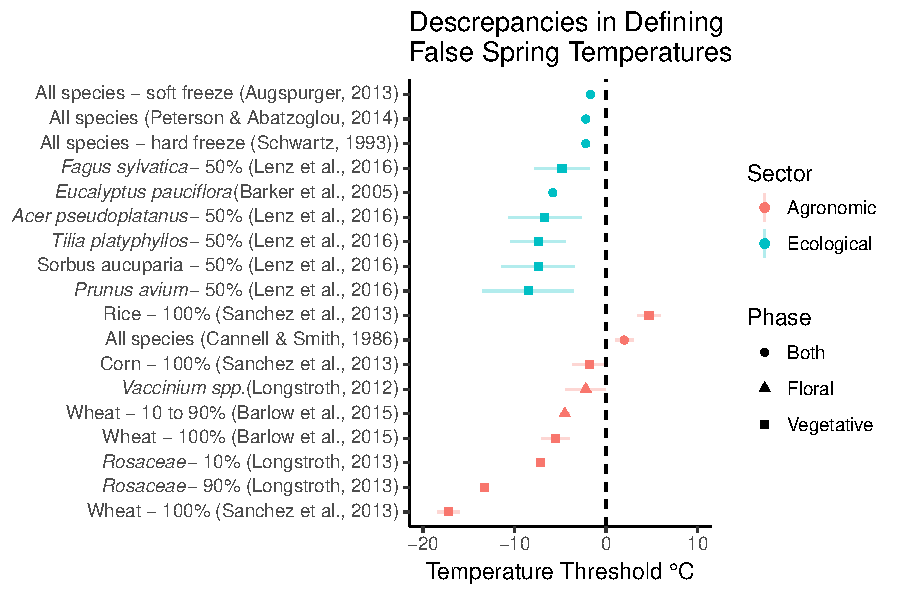
\includegraphics[width=\maxwidth]{figure/temp-1} 

}

\caption[A comparison of damaging spring freezing temperature thresholds across ecological and agronomic studies]{A comparison of damaging spring freezing temperature thresholds across ecological and agronomic studies. Each study is listed on the y axis along with the taxonimic group of focus. Next to the species name is the freezing definition used within that study (e.g. 100\% is 100\% lethality). Each point is the best estimate recorded for the temperature threshold with standard deviation if indicated in the study. The shape of the point represents the phenophases of interest and the colors indicate the type of study (i.e. agronomic or ecological).}\label{fig:temp}
\end{figure}



\begin{figure} [H] 
 -\begin{center}
 -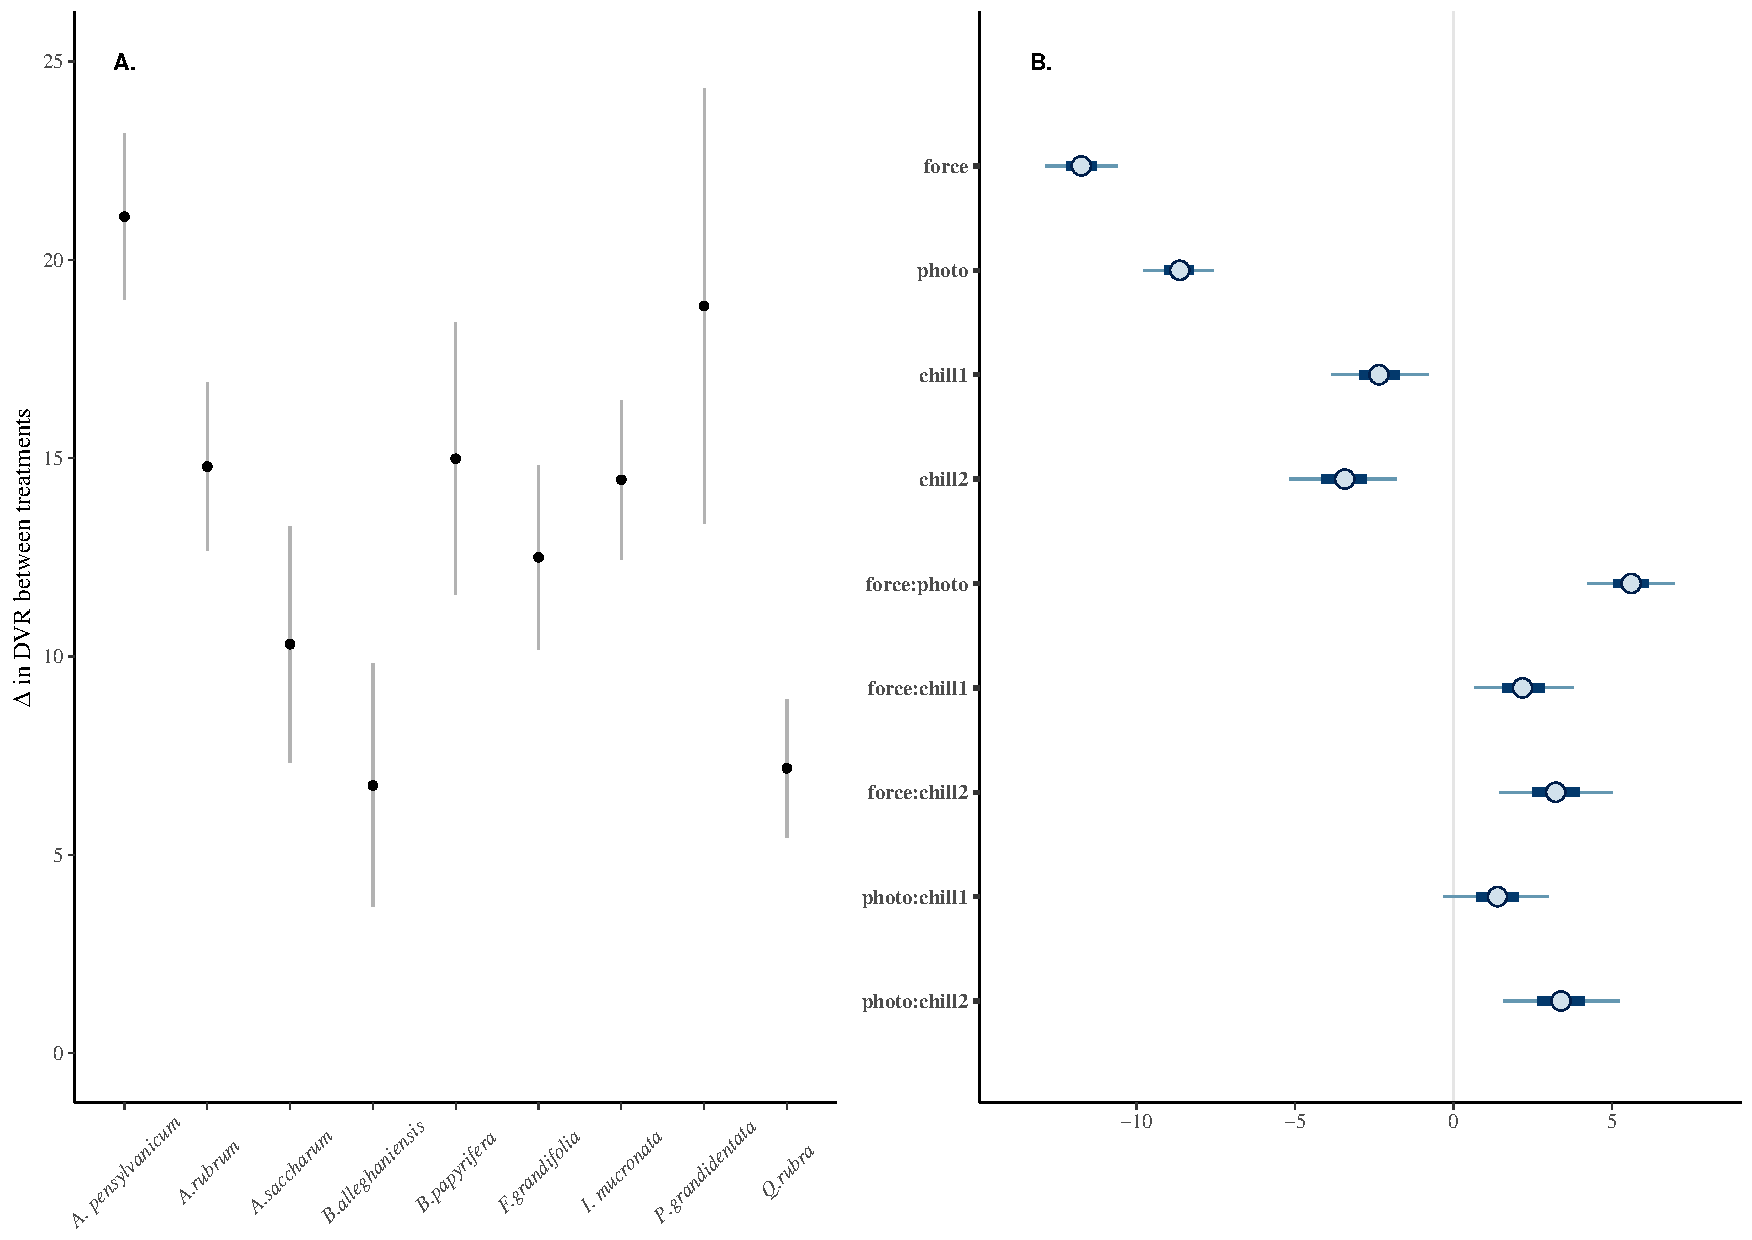
\includegraphics[width=16cm, height=13cm]{..//figure/DVRdiff_twoplots.pdf} 
 -\caption{Results from the growth chamber experiment. (A) A plot of the model parameter estimates on the duration of vegetative risk. Spring forcing temperatures had the largest effect on the rate of leafout, with photoperiod also being a critical factor. Thus, while greater forcing or longer photoperiods alone will shorten the duration of vegetative risk by 10 and 9 days respectively, their combined effect would be 14 days due to a 5 day delay through their interaction (10 + 9 - 5 = 14). Data was collected from a growth chamber experiment where one treatment had no additional overwinter chilling, low spring forcing temperatures, and shorter spring daylengths and the other had additional overwinter chilling, high spring forcing temperatures, and longer spring daylengths. (B) A comparison of the durations of vegetative risk across two treatments for each species collected for the experiment. Species along the x-axis are ordered by day of budburst. The standard error is represented by the bars around each point. }\label{fig:dan} 
 -\end{center}
 -\end{figure}
 
\begin{figure}[H]

{\centering 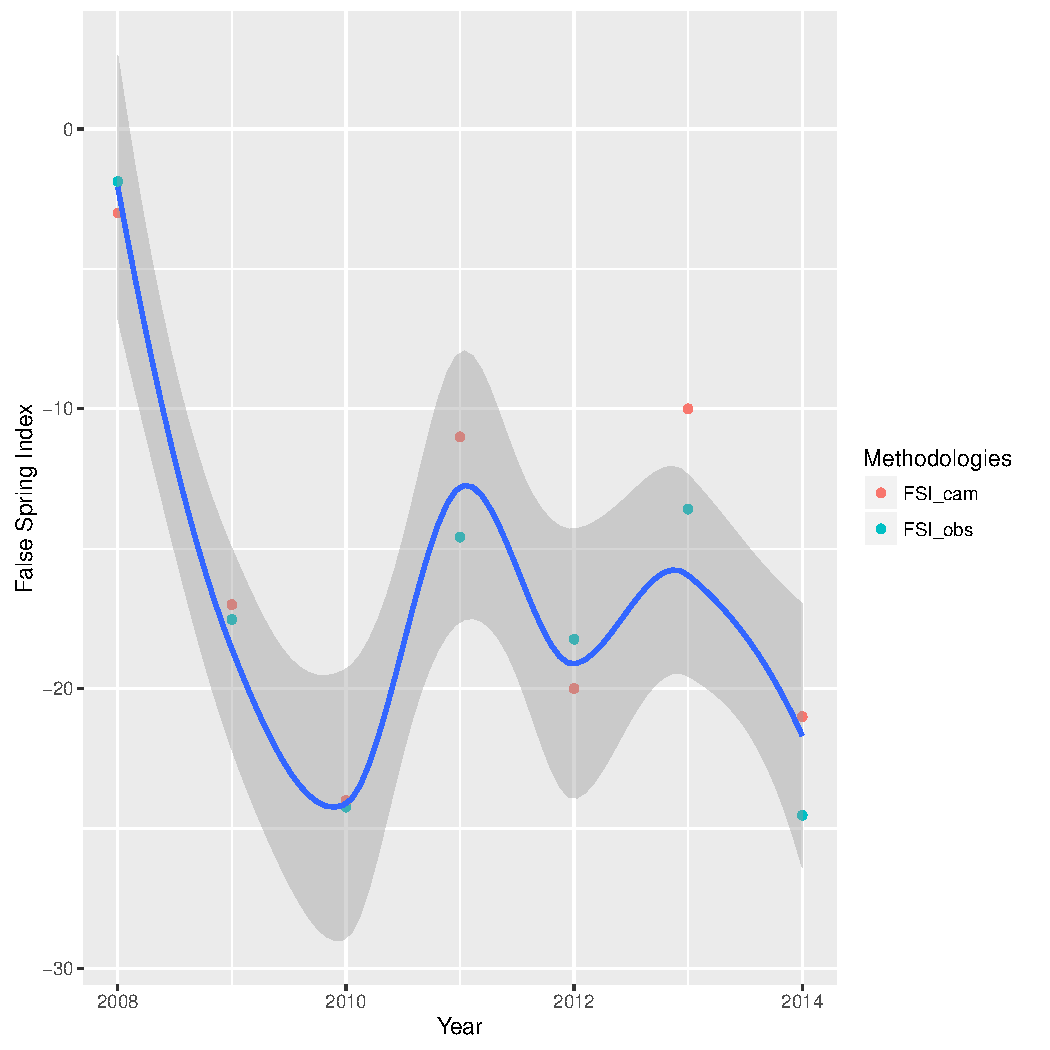
\includegraphics[width=\maxwidth]{figure/hf-1} 

}

\caption[Duration of vegetative risk for 8 species at Harvard Forest, comparing 1997 and 2012]{Duration of vegetative risk for 8 species at Harvard Forest, comparing 1997 and 2012. In 1997, the aggregated GDDs to budburst were the lowest and the durations of vegetative risk overall were shorter, whereas in 2012, the aggregated GDDs to budburst were the highest and the durations of vegetative risk were longer. The dotted line indicates a false spring event in 2012, which is defined as freezing temperatures (-2$^\circ$C) occurring after budburst. The histogram at the bottom right corner indicates the frequency of accumulated GDDs to budburst for each year between 1990 and 2016. It indicates that 1997 was a thermally late year and 2012 was a thermally early year. }\label{fig:hf}
\end{figure}



\begin{figure} [H] 
 -\begin{center}
 -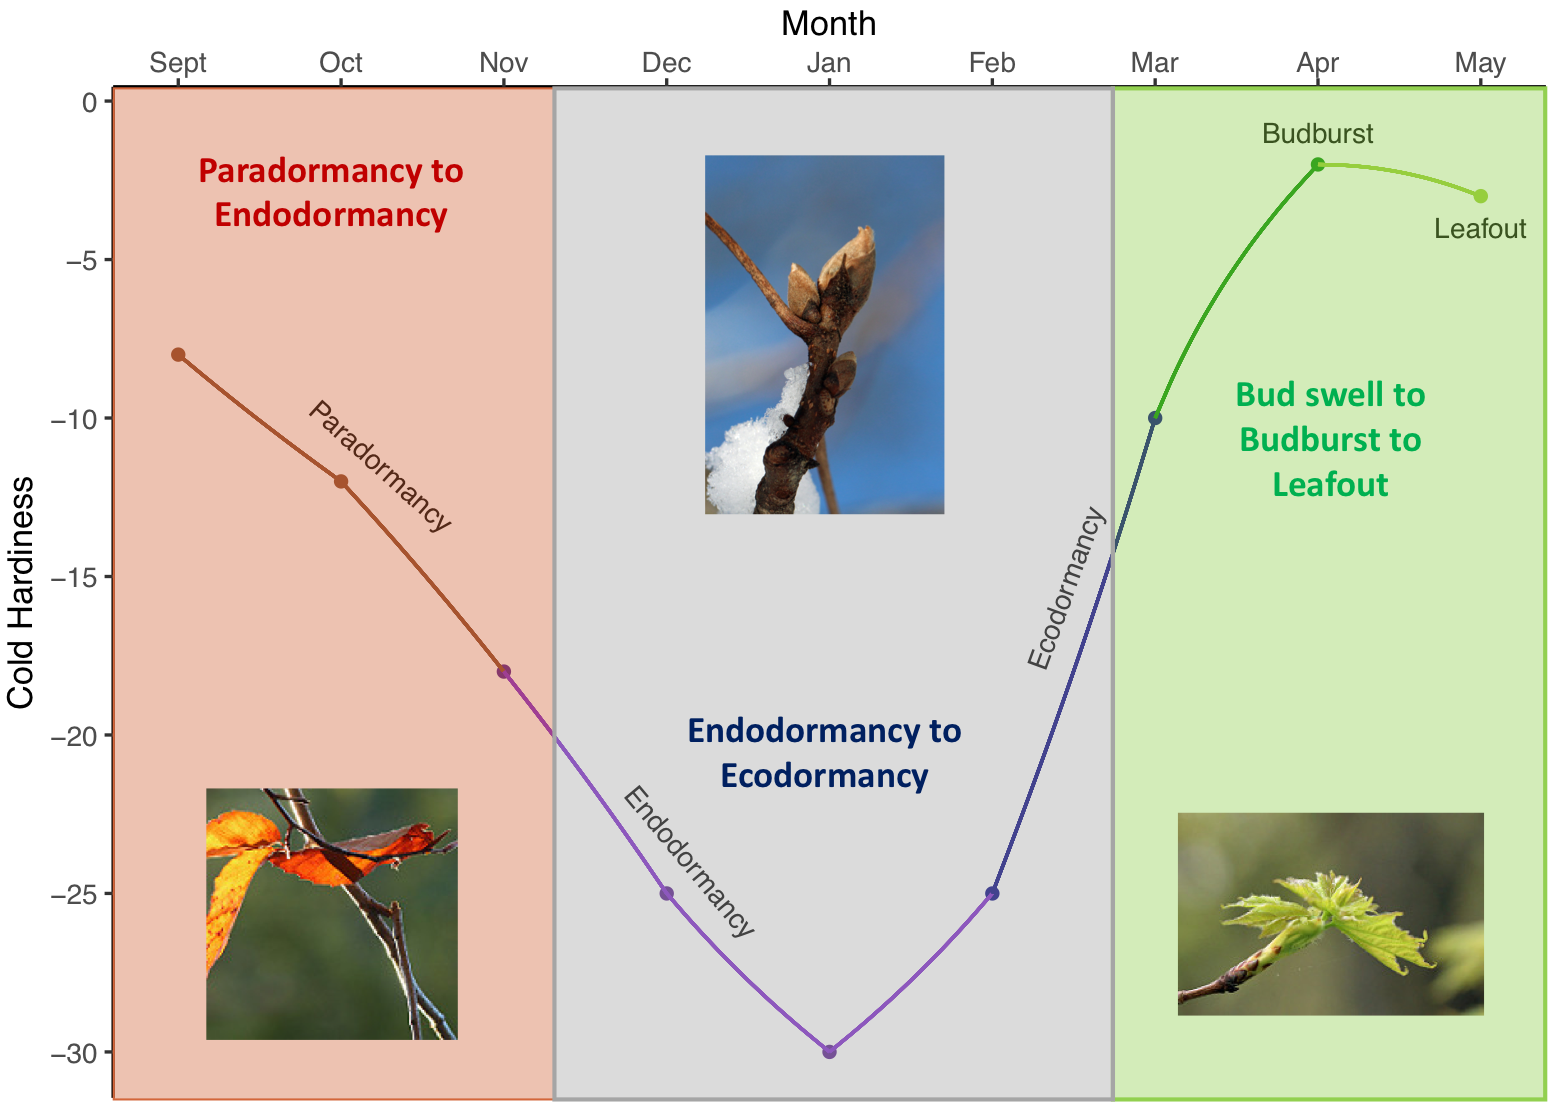
\includegraphics[width=16cm, height=13cm]{..//figure/hardinessfig_detailed.png} 
 -\caption{Frost tolerance (i.e. cold hardiness) in the fall increases rapidly as temperate plants begin to enter dormancy. Once buds reach the endodormancy phase, buds can tolerate temperates as low as -25$^{\circ}$C to -40$^{\circ}$C or lower (Charrier \& Am\'{e}glio, 2011, Vitasse et al., 2014). Frost tolerance diminishes again once buds begin to swell before budburst to around -8$^{\circ}$C and is lowest between budburst (-2$^{\circ}$) to leafout (-3$^{\circ}$). }\label{fig:hardiness} 
 -\end{center}
 -\end{figure}

\end{document}
